\documentclass[runningheads,a4paper]{llncs}
\usepackage{amssymb}
\usepackage[T1]{fontenc}
\usepackage[utf8]{inputenc}
\usepackage{graphicx}
\usepackage{wrapfig}
\usepackage{verbatim}
\usepackage{caption}
\usepackage{hyperref}

% #rubber: set arguments --shell-escape
\begin{document}


\title{Roofline Model applied to NUMA and Heterogeneous Memories}
\titlerunning{Roofline Model for Heterogeneous and NUMA Memories}
\author{Nicolas Denoyelle \and Aleksandar Ili\'{c}}
\institute{Inria - France -- INESC-ID -- Portugal\\
  Nicolas.Denoyelle@inria.fr, ilic@sips.inesc-id.pt}

\maketitle

\begin{abstract}
  The ever growing complexity of high performance computing systems, has made impossible for a single expert to master them
  entirely.
  %% In order to perform software optimizations several hardware abstraction models have been proposed to fit the system specificities
  .
  Recently, the Roofline Model has earned a great popularity modeling hardware and software, thanks to its simplicity and yet his
  efficiency. 
  %% This model has been successfully used to find some applications bottlenecks but also to estimate possible improvements limit.
  In this short paper we present an extended use of the traditional model, taking into account heterogeneous and NUMA memories
  in addition to the main DRAM memory.
\end{abstract}

\section{Introduction}
Emerging memory technologies (e.g non-volatile memory, heterogeneous memory architectures, on-package 
memory), are required to address applications' needs and improve the performance at the cost of a growing hardware complexity.
%% The next generation Xeon Phi processor will embed on-package memory, configurable as a hardware cache, or as 
%% a memory or both. This managable cache-memory mark the beginning of the use of on chip heterogeneous memory.
%% SMP systems with several memory nodes presents similar caracteristics, and were used to simulate heterogeneous memories, because
%% they also exhibit non uniform memory accesses.

The memory wall makes data locality increasingly important, especially in this context, to achieve good performance.
We think we can leverage the Roofline Model to detect some data locality issues related to memory bandwidth.
For instance, a data allocated on low-bandwidth memory, may lead the application to become bandwidth bound.
Our extension to heterogeneous and NUMA memory shows that in such sytems, memory bandwidth may vary from one pair
(source, destination) to another.
Thus bad data locality can be spotted by observing those bandwidth bounds reached by an application.

%% Further more, this model has been successfully used to demonstrate application optimizations in several papers, and will
%% probably be implemented as a feature in the Intel advisor tool.

The remainder of this paper is organized as follow:

The section~\ref{sec:state_of_art} will describe the model and the most interesting existing improvements.
Finally section~\ref{sec:contrib} will briefly describe our implementation to measure memory bandwidths, and the validation of the model.

\section{The Roofline Model Then and Now}
\label{sec:state_of_art}

\begin{wrapfigure}{R}{40mm}
  \centering
  \includegraphics[width=30mm]{pictures/model_drawing}
  \caption{Roofline model draw}
  \label{fig:roofline_draw}
\end{wrapfigure}

The original paper~\cite{Williams:2009:RIV:1498765.1498785} depict a machine with two subsystems: a memory and a compute unit,
running the instructions dispatched from a common instruction channel.

This idea is drawn on figure~\ref{fig:roofline_draw}.
Depending on the operational intensity (i.e. the ratio of compute instructions over memory instructions),
one unit, the other or both may be saturated with instructions. The width of the memory channel is the bandwidth and the width
of the compute channel is the fpeak (floating point peak) performance. The model assumes there can be no dependency between
instructions (they can overlap perfectly) and instructions' lattency is hidden.

On figure~\ref{fig:orig_model} is shown the graphical representation of the model.
The operational intensity stands on abscissa and the performance stands on the ordinate axis.
Top horizontal lines show the fpeak performance for different type of compute instructions and
oblique lines show the memory bandwidth for different types of memories. On this representation
one can see that: the roofline model ($min(bandwidth*operational\_intensity, fpeak)$) shows whether a pattern of compute/memory
instructions interleaving is either compute or memory bound.

The model has been successfully used in
several~\cite{Kim20111201}~\cite{Rossinelli2164}~\cite{vanNieuwpoort:2009:UMH:1542275.1542337} application optimizations, whether
to prove bottlenecks, or measure achievable (or achieved) improvements.

It has been applied to other memory subsystems~\cite{ilic2014cache}, energy~\cite{7493653}, and abstract runtime systems.

Based on the Cache Aware Roofline Model methodology, we applied and validated the model to heterogeneous memory subsystems.

\section{Contribution}
\label{sec:contrib}

In our contribution, we developped a tool able to benchmark rooflines and validate them with micro kernels, compatible with intel chips.

Each benchmark (rooflines, and micro kernels) is made of assembly code using best architectures instructions available at compile
time.

In brief, the compute benchmark repeats compute instructions and outputs $\frac{n*iFlops}{time}$ where $n$ is the number of compute instructions and $iFlops$ is the number of floating point operations computed per instruction.

The memory benchmark repeats coallesced memory instruction on a private\footnote{Each thread have its own buffer's chunk} buffer of several sizes fitting the memory to benchmark and outputs $\frac{n*iBytes}{time}$ where $n$ is the number of memory instructions and $iBytes$ is the number of Bytes transferred per instruction.

We can find several arithmetic floating point operation peaks (addition, multiplication, overlapping multiply add, and fuse
multiply add), as well as several bandwidth types (load, store, non temporal load, non temporal store, interleaving of 2 loads and one store), and for several memory levels (L1, L2, L3, (caches \dots), NUMA memories, MCDRAM \dots) detectable with hwloc~\cite{6903671} library.

\begin{figure}
  \centering
  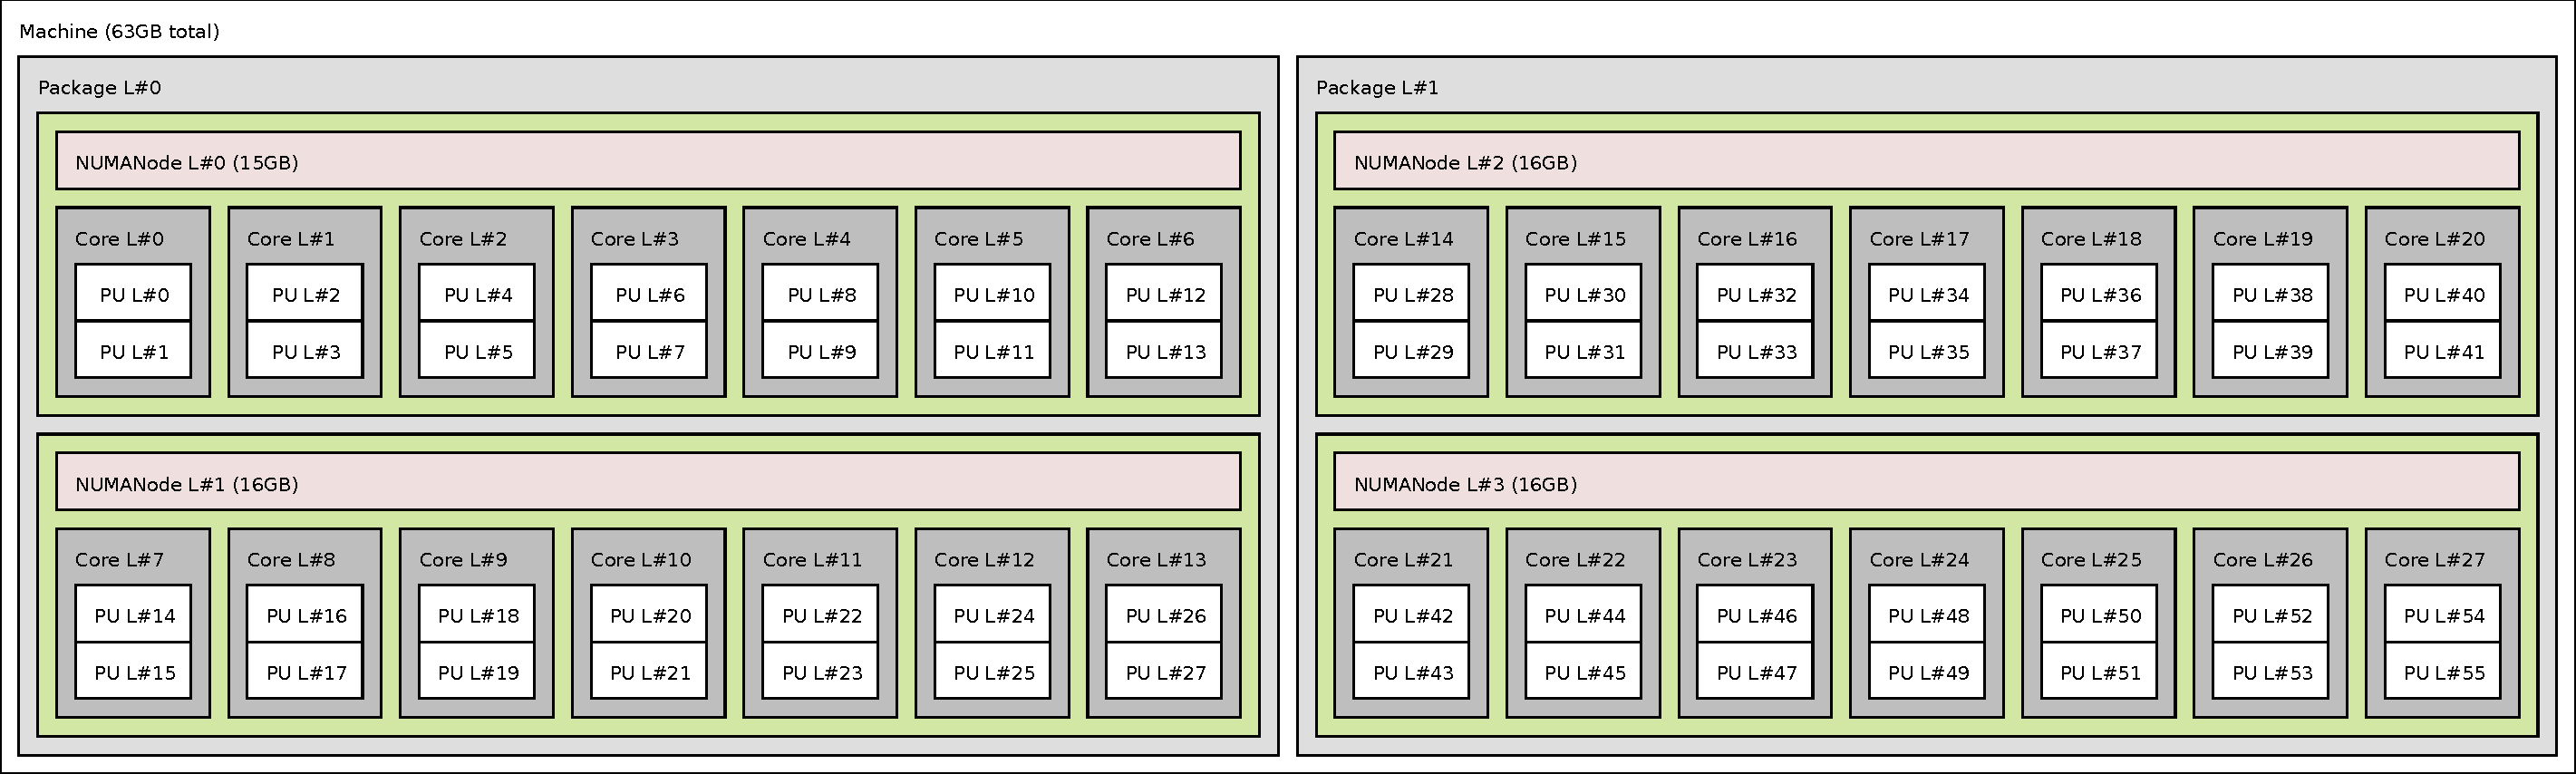
\includegraphics[width=\textwidth]{pictures/Xeon_E5_2650L_v4}
  \caption{Machine topology, with hidden caches}
  \label{fig:joe0}
\end{figure}

Figure~\ref{fig:joe0} shows a represtentation of such a machine given by hwloc, in the form of nested boxes representing
hierarchical inclusiveness of ressources in the machine. Our benchmark can work both in sequential and in parallel. In the former,
one benchamrk thread is spawn on first Core (left most) of the machine. In the latter, one benchmark thread per Core of the first
NUMA memory node is spawn, and threads measure (Flops and Bytes) are accumulated. The parallel model representation obtained from
machine~\ref{fig:joe0} is shown on figure~\ref{fig:orig_model}. In this model sum of each thread load bandwidth on its (non-shared)
 L1 cache yields a throughput of 761GB/s, whereas the shared local memory (NUMANode:0) yields a throughput of 36GB/s.
Remote memory bandwidth are obtained by running the same benchmark as local memory, but explicitly allocating the data on remote
 memories.
On this figure, the lines shows the top measures, and one can notice, on L3 a wider line with less opacity showing the measured
bandwidth deviation.
We can also notice that for L1 (black line), the points does not stick very well to lines around the ridge. Actually the points
does not measure the bandwidths, but instead validate rooflines. They consist of micro kernels of different known operational
intensities, interleaving memory and compute instruction to reach rooflines, and show how realistic the model is with those
metrics, by measuring each kernel's performance.

\begin{figure}
  \centering
  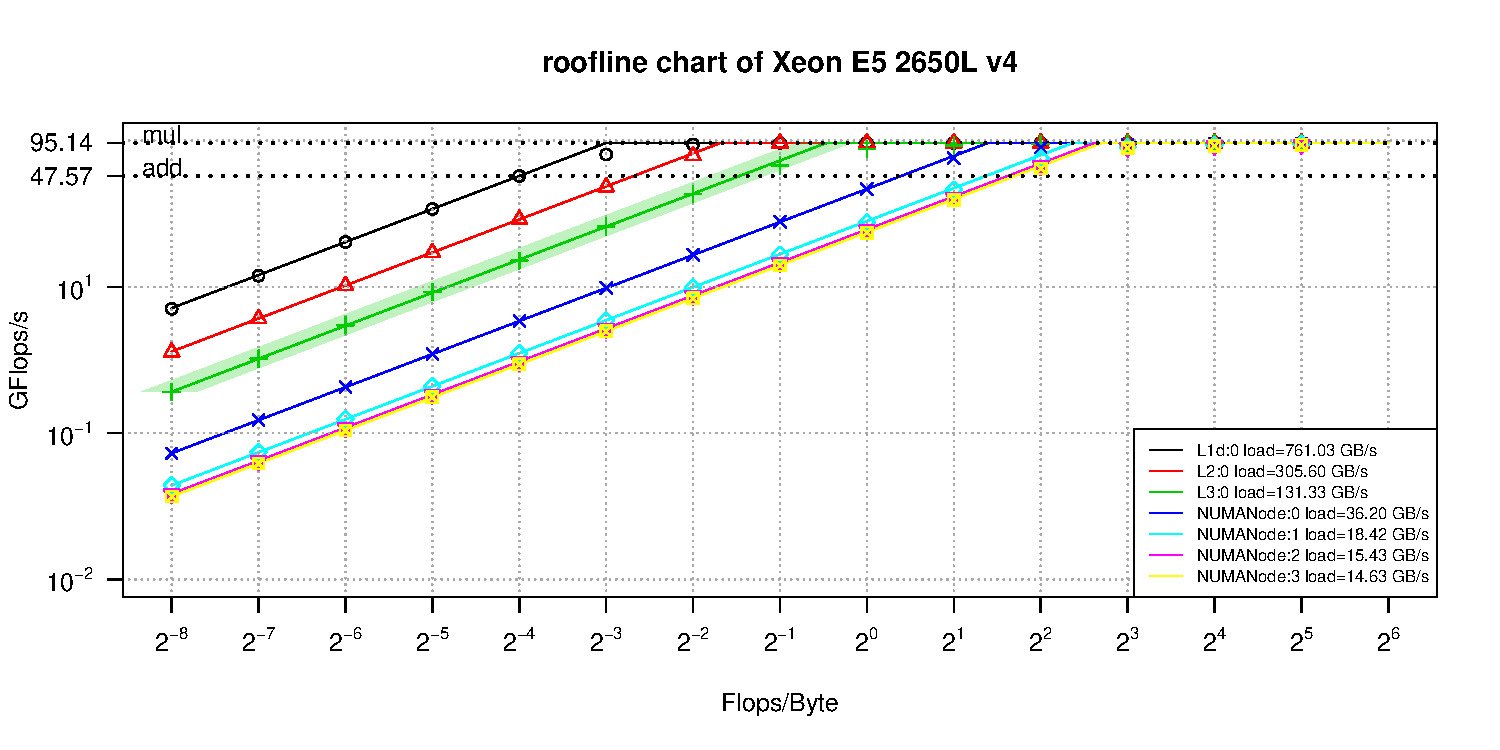
\includegraphics[width=\textwidth]{pictures/roofline_model}
  \caption{Example of the original roofline chart}
  \label{fig:orig_model}
\end{figure}

%% Our benchmarks consists in several hand written micro code to maximize the throughput of floating point, 
%% load and store instructions. 
%% Each measure is taken 16 time and we retain the median instruction 
%% throughput result to filter unexpected behaviours.
%% We take care of using every available register for each kernel, and minimize the reuse of each, to 
%% minimize dependencies. Each benchmark has a loop structure allowing to run it arbitrarily long to drown the
%% measure overhead and allow sampling of each single benchmark. 
%% This allows to match hardware counters gathered with some external sampling tool, with the counted values.

%% Each benchmark uses intel best SIMD instructions available at compile time.
%% Therefore the benchmark can only work (for now) on intel compatible cpus.
%% Instruction count is known at runtime, as well as the bytes transfered and flops performed for each instruction.
%% Hence the only thing to measure, in order to get performance and bandwidth, are the cycles elapsed.

%% Timestamps are taken with the pair CPUID/RDTSC instructions[1],
%% then time is computed using the set cpu frequency.  
%% The timestamp instruction are direcly written in the assembly benchmark in sequential code to avoid that the
%% compiler insert more instructions in between timestamps and benchmark. 
%% Parallel code cannot use the same technique because we read timestamp counter before the start barrier 
%% and after the end barrier to assert simultaneous start and total completion when taking timestamp. 
%% Hence an openmp runtime overhead is applied, but before the proximity of results between parallel and 
%% sequential code, we avoided heavy overhead measures.

%% The floating point benchmark basically interleave SIMD multiplications and additions.
%% This achieves better performance than only additions or only multiplications because those to kind of operation
%% can often be performed simultaneously.

%% The bandwidth benchmark serializes SIMD load or store instruction, but never make use of the data. 
%% This is because we aim to get the machine very top upper bound, instead of getting upper bound with realistic 
%% code, matching even assembly level optimizations.
%% (We started to develop a generic benchmark written in realistic C code already. Maybe released later, and 
%% result maybe here also later).
%% For this benchmark we allocate once a buffer of 16 times the Last Level Cache (LLC) size.
%% For each memory in the hierarchy (including caches) we cut it into 4*N (N is the number of threads) times the 
%% above memory size, to the current memory size. 
%% Each buffer slice we bench, is both a multiple of N to be split among all threads and a multiple of the 
%% minimum chunk size to be used for the bandwidth benchmark kernel (one of the reasons lie into vector
%% sizes which impose a minimum block size). 
%% Each thread chunk of data cannot fit above memory.
%% Each then load its chunk of data using different sizes, for each memory level and each memory node (NUMA)
%% as detected by hwloc. For a given memory (level or node) we keep one sample among of all benchmark samples
%% which is again the median instruction throughput value, and the standard deviation of it.
%% When the data chunk is greater than LLC size, we use non-temporal store instructions better suited for 
%% streaming workloads, by-passing the caches and avoiding a read for ownership.

%% The validation kernels are dynamically written, compiled and run, depending on input operational intensity.
%% They interleave instructions from fpeak and bandwidth benchmarks such that they are uniformly spread 
%% into the loop, and such that each register reuse is minimized. The same method used for bandwidth benchmark is 
%% used to determine buffer size, and benchmark result.

%% We use hwloc[2] to gather the necessary machine topology informations.
%% We use openmp runtime to parallelise the benchmark.

%% Whether we use hyperthreading or not we set the number of threads to the number of hardware threads(PU) or to 
%% the number of Core under the very first memory node. 
%% Afterward, each thread will bind to the PU/Core corresponding to its openmp thread id.

%% The cpu frequency is input by user via environment variable, or taken from /proc/cpuinfo if not.
%% The cpu frequency is actually very hard to measure[3] and we set it manually to get relevant results.
%% Turboboost technology was of course disable for the experiments.

\section{Conclusion and future work}

In this short paper we prestented the Roofline Model and an extension to heterogneeous memory's sytem using the Cache Aware
Roofline Model methodology. Later on we will validate the interest of this representation with applications. 


\bibliographystyle{splncs03}
\bibliography{references}

\end{document}

